
\subsection{The package of GUI}

\subsubsection{UserInterface Controller and UserInterface Player}

The first FXML interface controller is responsible for the main scene and communicates with the logic package. Any performance of the users is exhibited on this primary User Interface, for example, players can operate the game, select the provided options on the menu bar, and observe the current game situation. 

For the second scene UserInterfacePlayer, it manages the initialization of the state of participants. Players can manually insert their names and decide which players will be played by the bot. 

With regards to the communication of these two windows as the Figure \ref{fig:guiPackage} below, the first interface establishes a reference of the second window in order to getter method to pass players' names and states to the main window. 
It can clearly conclude that it is a one-direction for passing information from the first scene to the second scene. 


\begin{figure}[h]
	\centering
	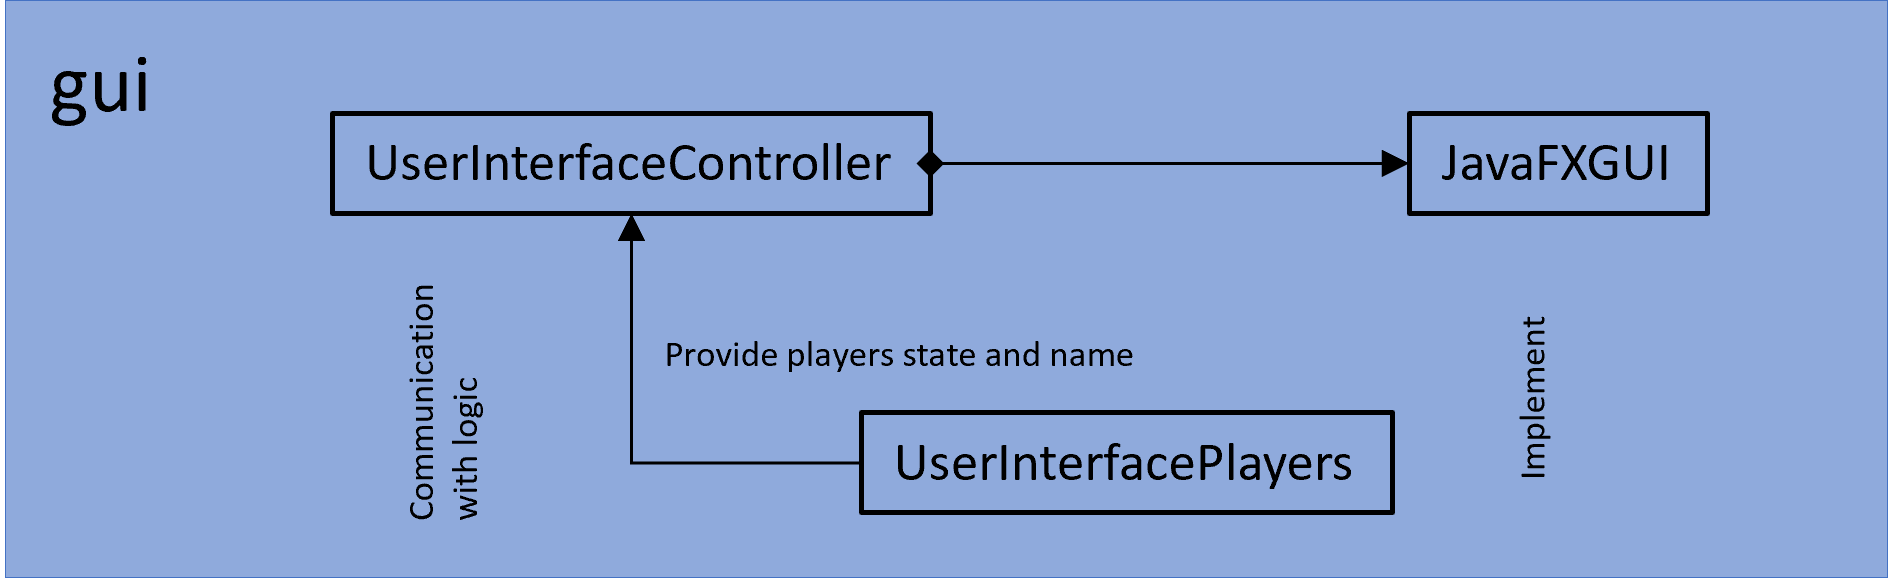
\includegraphics[width=0.8\textwidth]{image/diagram_2}
	\caption{The GUI package}
	\label{fig:guiPackage}
\end{figure}

\subsubsection{JavaFxGUI}
The aims of all the methods in JavaFxGUI allow the logic class to change the output GUI. In fact, the JavaFxGUI can be implemented by the class GUIConnector, which is being used in the logic package. For example, while the logic class needs to modify the chessboard by placing a symbol token, it is undoubtedly that the display of the interface also needs to update the game field simultaneously. 
Thus, the function of the class JavaFxGUI can be utilized for this purpose. 